\begin{center}
\fbox{\fbox{\parbox{6.5in}{\centering
\begin{flushleft}
\hspace{5mm}
\textbf{\underline{Kiiruse valem}}\\
\vspace{5mm}
\hspace{5mm}
Kiirus ütleb meile, kui suure vahemaa/teepikkuse me läbime mingis kindlas ajaühikus.\\
\vspace{2mm}
\hspace{5mm}
Seega kiiruse valem: \fbox{$v=\dfrac{s}{t}$} \hspace{2mm}, kus $v$ - \textbf{kiirus}, $s$ -\textbf{teepikkus} , $t$ - \textbf{aeg}.\\
\vspace{2mm}
\hspace{5mm}
Kiiruse valemist on võimalik tuletada ka teepikkuse ja aja valemid.\\
\vspace{2mm}
\hspace{5mm}
\textbf{Teepikkus: } \fbox{$s=v\cdot t$} \hspace{5mm} \textbf{Aeg: } \fbox{$t =\dfrac{s}{v}$}\\
\vspace{5mm}
\hspace{5mm}
Näiteks, olgu meil $s=125$m ning $v=25$m/s. Leiame aja $t$:\\
\vspace{2mm}
\hspace{5mm}
$t=$ $\dfrac{125\hspace{0.5mm}m}{25\hspace{0.5mm}m/s}=\dfrac{125}{25}\cdot \dfrac{m}{m/s}=5\cdot \left( m:\dfrac{m}{s}\right)=5\cdot \left(\dfrac{m}{1}\cdot \dfrac{s}{m}\right)=5\cdot \left(\dfrac{\cancel{m}\cdot s}{1 \cdot \cancel{m}}\right)=5 \cdot \dfrac{s}{1}=5 \hspace{0.5mm}s$\\
\vspace{5mm}
\hspace{5mm}
\textbf{\underline{Aja-teepikkuse graafik}}\\
\vspace{2mm}
\hspace{5mm}
Olgu meil järgmine graafik (Joonis \ref{t ja s}).
\begin{center}
    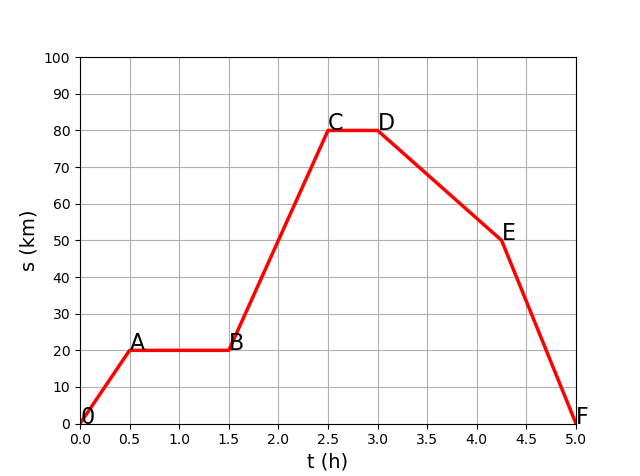
\includegraphics[width=8cm]{aeg-teepikkuse graafik.png}
    \captionof{figure}{Aja ning teepikkuse graafik}
    \label{t ja s}    
\end{center}
\vspace{2mm}
\hspace{5mm}
Selliste spetsiifiliste graafikute puhul tuleb alati endale kindlaks teha, mida näitab meile $x$-telg ning\\
\hspace{5mm} mida $y$-telg? Praegusel juhul näitab $y$-telg teepikkust $s$ kilomeetrites ning $x$-telg näitab meile aega $t$\\ \hspace{5mm} tundides. Näeme ka, et kui liikuda mööda $x$-telge paremale, siis suureneb aja $t$ väärtus. Kui liikuda\\ \hspace{5mm} mööda $y$-telge suunaga ülesse, siis suureneb meil teppikkus $s$.\\
\vspace{2mm}
\hspace{5mm}
Kui liigume mööda punast joont, siis märkame, et punktist 0 punkti A jõudmiseks pidime läbima 20\\ \hspace{5mm} km (sest 0 ja A vaheline kaugus $y$-telje järgi on 20 ühikut). Kuid kui uurida sama liikumist $x$-telje\\ \hspace{5mm} järgi, siis näeme, et punktist 0 punkti A jõudmiseks kulus meil 0.5 tundi (Pane tähele! Kilomeeter\\ \hspace{5mm} vs tund!). Ehk piltlikult öeldes, me kasutame punktist 0 punkti A liikumise kirjeldamiseks kahte\\ \hspace{5mm} erinevat mõõdupuud/joonlauda. Ühel joonlaual on ühikuteks tunnid ning teisel joonlaual ühikuteks\\ \hspace{5mm} kilomeetrid.\\
\vspace{2mm}
\hspace{5mm} Näide jätkub järgmisel lehel...

\end{flushleft} }}}
\end{center}



\newpage


\begin{center}
\fbox{\fbox{\parbox{6.5in}{\centering
\begin{flushleft}


\hspace{5mm}
Saadud andmetega, saame leida ka liikumise kiiruse: $v=\dfrac{s}{t}=\dfrac{20\hspace{0.5mm} km}{0.5 \hspace{0.5mm}h}=\dfrac{200}{5}\cdot \dfrac{km}{h}=40\cdot \dfrac{km}{h}=40 km/h$.\\
\vspace{1mm}
\hspace{5mm}
Uurime liikumist punktist A punkti B. Möödunud ajaks on meil 1 tund (0.5 pealt läheb 1.5 peale), kuid\\ \hspace{5mm} teepikkus jääb 20 km peale pidama. Kuna läbitud teepikkus punktis B on sama, mis oli eelmises\\ \hspace{5mm} punktis A, siis oleks loomulik järeldada, et mingit liikumist meil tegelikult ei toimunudki. Ehk tund\\ \hspace{5mm} aega meil küll möödus, aga läbitud teepikkus ei muutunud. Kuna läbitud teepikkus ei muutunud, siis\\ \hspace{5mm} on lõigul AB läbitud teepikkuseks $s=0\hspace{0.5mm}km$. Läbitud aeg $t=1 \hspace{0.5mm}h$. Järelikult kiirus: $v=\dfrac{s}{t}=\dfrac{0}{1}=0km/h$.\\
\hspace{5mm}
See on loomulik, sest kui me oleme paigal ja kuhugi ei liigu, siis ei saa meil ka kiirust olla.

\end{flushleft} }}}
\end{center}


\vspace{1cm}

\textbf{Märkmed}\\
\vspace{2mm}
\begin{mdframed}[style=graphpaper]
\vspace{14cm}
\end{mdframed}